%Dave's handout 1.7 intro 2nd derivatives
%Dave's handout 2.2 2nd derivative rule
\vspace{-0.25 in}
\begin{framed}
\subsection*{Objectives}
\begin{itemize}
    \item Define absolute extrema and local extrema.
    \item Use first derivative test and second derivative test to find local extrema.
    \item Locate absolute extrema over a closed interval.
\end{itemize}

%%%Reading Assignment%%%
\subsection*{Suggested Reading:}
\begin{itemize}
\item \cite{Calaway}\footnotemark[1]
   \begin{itemize}
        \item \emph{Section 2.7 Optimization}
    \end{itemize}
\end{itemize}
%\subsection*{Supplemental Materials:}
%%%Key Terms%%%
\subsection*{Key Terms and Concepts:} 

\begin{multicols}{2}
\begin{itemize}
    \item Partition Numbers vs. Critical Numbers
    \item Sign Chart
    \item First Derivative Test
    \item Second Derivative Test
    \item Local Maximum and Local Minimum
    \item Absolute Maximum and Absolute Minimum
\end{itemize}
\end{multicols}
\end{framed}
\footnotetext[1]{Available free to download from \url{http://www.opentextbookstore.com/details.php?id=14} .}

\newpage
%%%%%%%%%%START LESSON CONTENT%%%%%%%%%%%%%
%\noindent\makebox[\linewidth]{\rule{\textwidth}{0.8pt}}
\Opensolutionfile{ans}[ans8]
\Opensolutionfile{ansL}[ansL8]
%%%%%%%%%%%%%%%%Start First Topic%%%%%%%%%%%%%%%%%%%%%%%%%%%%%
\noindent Without calculus, we only know how to find the optimum points in a few specific examples (for example, we know how to find the vertex of a parabola). But what if we need to optimize an unfamiliar function?\\
The best way we have without calculus is to examine the graph of the function, perhaps using technology. But our view depends on the viewing window we choose – we might miss something important. In addition, we’ll probably only get an approximation this way. (In some cases, that will be good enough.)\\
Calculus provides ways of drastically narrowing the number of points we need to examine to find the exact locations of maximums and minimums, while at the same time ensuring that we haven’t missed anything important.\\
Before we examine how calculus can help us find maximums and minimums, we need to be familiar with the vocabulary and the concepts we will develop and use to describe \textbf{behavior of a function}.\\

\begin{tcolorbox}[title = {Increasing and Decreasing Functions in an interval}]
    Simply put, if there is some interval of values of x for which the value of a function is getting larger as we move from left to right, we say that the function is increasing in that interval.  A decreasing function is defined similarly, with the value of the function becoming smaller vs. larger.\\\\
    For a function \(f\) which is \emph{differentiable}\footnotemark on an interval \(I\):
\renewcommand{\labelenumii}{\roman{enumii}}
\begin{enumerate}
    \item if \(f'(x)>0\) for all \(x\) in the interval \(I\), then \(f\) is \textbf{increasing} on \(I\).
     \item if \(f'(x)<0\) for all \(x\) in the interval \(I\), then \(f\) is \textbf{decreasing} on \(I\).
      \item if \(f'(x)=0\) for all \(x\) in the interval \(I\), then \(f\) is \textbf{constant} on \(I\).
\end{enumerate}
\end{tcolorbox}

\noindent The derivative of a function tells about the general shape of the function, and we can use that shape information to determine if an extreme point is a maximum or minimum or neither (See Figure \ref{fig:dervBeh2}).

\begin{figure}[h]
    \centering
    \caption{} \footnotemark
    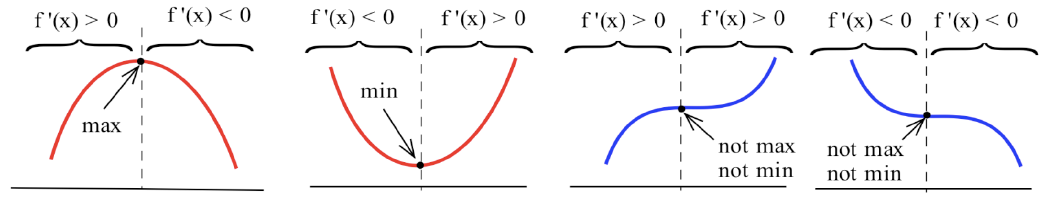
\includegraphics[width=0.95\textwidth]{derivatives-functions/derivativeBehavior} 
    \label{fig:dervBeh2}
\end{figure}

\footnotetext[1]{See Lesson \ref{differentiability}: Differentiability and Continuity}
\footnotetext[2]{From \cite{Hoffman} ;  page 88}

\subsection*{Extreme Points}

\begin{tcolorbox}[title = {Local Extreme Points }]
\begin{itemize}[leftmargin=*]
    \item A \textbf{local maximum} point is a point on the graph of the function at which the function changes from an increasing function to a decreasing function. A point is a local maximum if it is \underline{higher than} all the \textbf{nearby points}. Formally, we say
    \begin{itemize}
        \item $f$ has a \textbf{local maximum} at $c$ if $f(c)\ge f(x)$ for all $x$ near $c$.
    \end{itemize}
    \item A \textbf{local minimum} point is a point on the graph of the function at which the function changes from a decreasing function to an increasing function. A point is a local minimum if it is \underline{lower than} all the \textbf{nearby points}. Formally, we say
    \begin{itemize}
        \item $f$ has a \textbf{local minimum} at $c$ if $f(c)\le f(x)$ for all $x$ near $c$.
    \end{itemize}
\end{itemize}
\end{tcolorbox}
\vspace{-0.5cm}
\subsubsection*{Notes:}
\begin{itemize}
    \item These points are also referred to as “relative” maximum and minimum points.
    \item $f$ has a \textbf{local extremum} at $c$ if $f(c)$ is a local maximum or minimum. The plural of local extremum is \textbf{local extrema}.
    \item The plurals of these are \textbf{maxima} and \textbf{minima}. We often simply say \textbf{“max”} or \textbf{“min”}.
    \item The process of finding \emph{maxima} or \emph{minima} is called \textbf{optimization}.
\end{itemize}
\vspace{1in}
\begin{tcolorbox}[title = {Global Extreme Points }]
\begin{itemize}[leftmargin=*]
\item A \textbf{global maximum} point is the point at which the largest value of the function occurs.Formally, we say
    \begin{itemize}
        \item $f$ has a \textbf{global maximum} at $c$ if $f(c)\ge f(x)$ for all $x$ in the domain of $f$.
    \end{itemize}
\item A \textbf{global minimum} point is the point at which the smallest value of the function occurs. Formally, we say
    \begin{itemize}
        \item $f$ has a \textbf{global minimum} at $c$ if $f(c)\le f(x)$ for all $x$ in the domain of $f$.
    \end{itemize}
\end{itemize}
\end{tcolorbox}
\vspace{-0.5cm}
\subsubsection*{Notes:}
\begin{itemize}
    \item These points are also referred to as “absolute” maximum and minimum points.
    \item Every global extreme is also a local extreme but there are local extremes that are NOT global extremes.
\end{itemize}
\vspace{-0.5cm}
\begin{figure}[h]
    \centering
    \caption{} 
    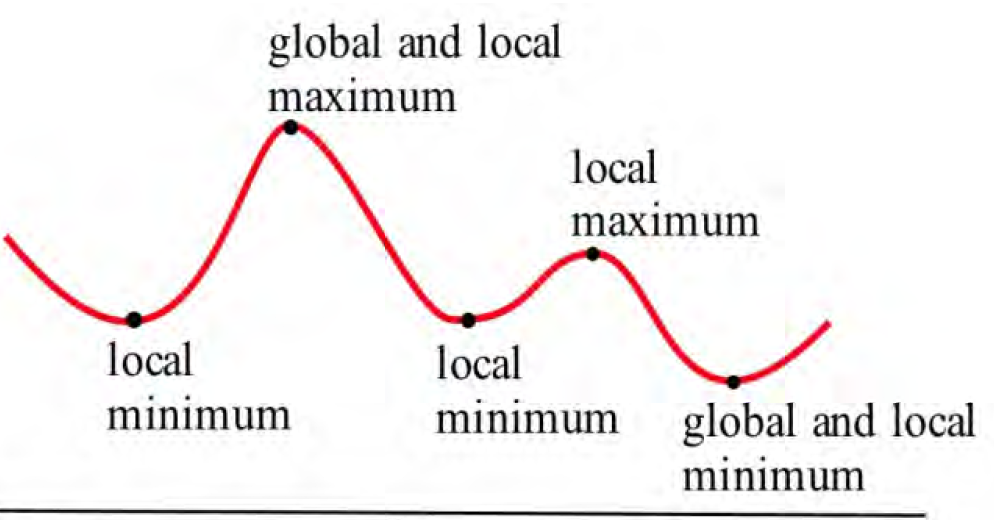
\includegraphics[scale=0.4]{images/optimization/globalVSlocalExtrema.png} 
    \label{fig:globalVSlocalExtrema}
\end{figure}
\newpage
\subsection*{Finding Maxima and Minima of a Function}
\begin{tcolorbox}[title = {A Partion Number, Critical Number and A Critical Point}]
\begin{itemize}[leftmargin=*]
    \item A \textbf{partition number} of $f'$ is a number $p$ for which either $f'(p)=0$ or $f'(p)$ is undefined.
    \item A \textbf{critical number} of a function $f$ is a number $c$ for which either $f'(c)=0$ or $f'(c)$ is undefined \underline{AND $c$ is in the domain of $f$}.
    \item A \textbf{critical point} of a function $f$ is a point $(c,f(c))$ where $c$ is a critical number of $f$.
    \begin{itemize}
        \item See the point marked by an arrow in figure \ref{fig:dervBeh2}, where $f'(x)=0$ and $f'(x)$ is undefined. 
    \end{itemize}
\end{itemize}
\end{tcolorbox}
\vspace{-0.5cm}
\subsubsection*{Notes:}
\begin{itemize}
    \item Critical numbers are also partition numbers, but partition numbers may not be critical numbers.
    \item A local max or min of $f$ can only occur at a critical point.
    \item The critical numbers only give the \textbf{possible} locations of extremes, and some critical numbers are not the locations of extremes.
    \item If the function has only one critical point and it’s a local max (or min), then it must be the global max (or min). 
    \begin{figure}[h]
    \centering
    \caption{} 
    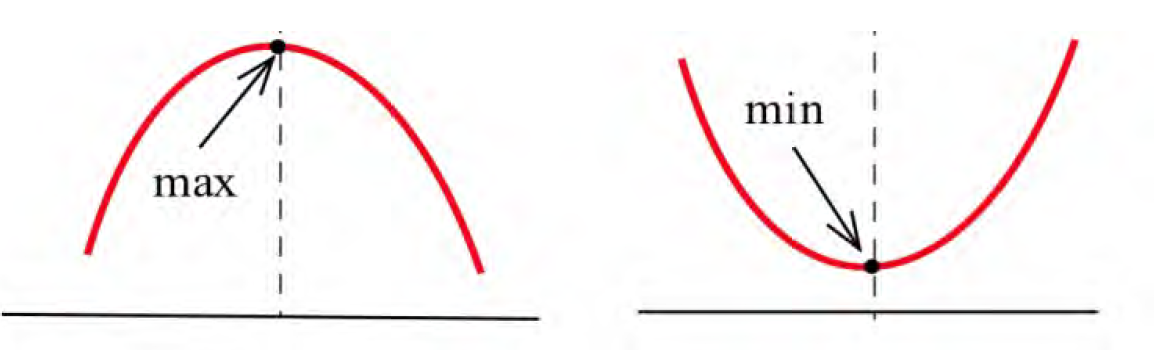
\includegraphics[scale=0.45]{images/optimization/oneLocalExtrema.png} 
    \label{fig:oneLocalExtrema}
\end{figure}
    
\end{itemize}
%%%%%%%%%%%%%%%%%%%%%%%%%%%%%%%%%%%%%%%%%
\begin{figure}[h]
\centering
    \caption{Different possibilities for critical points and corresponding local extrema.} 
    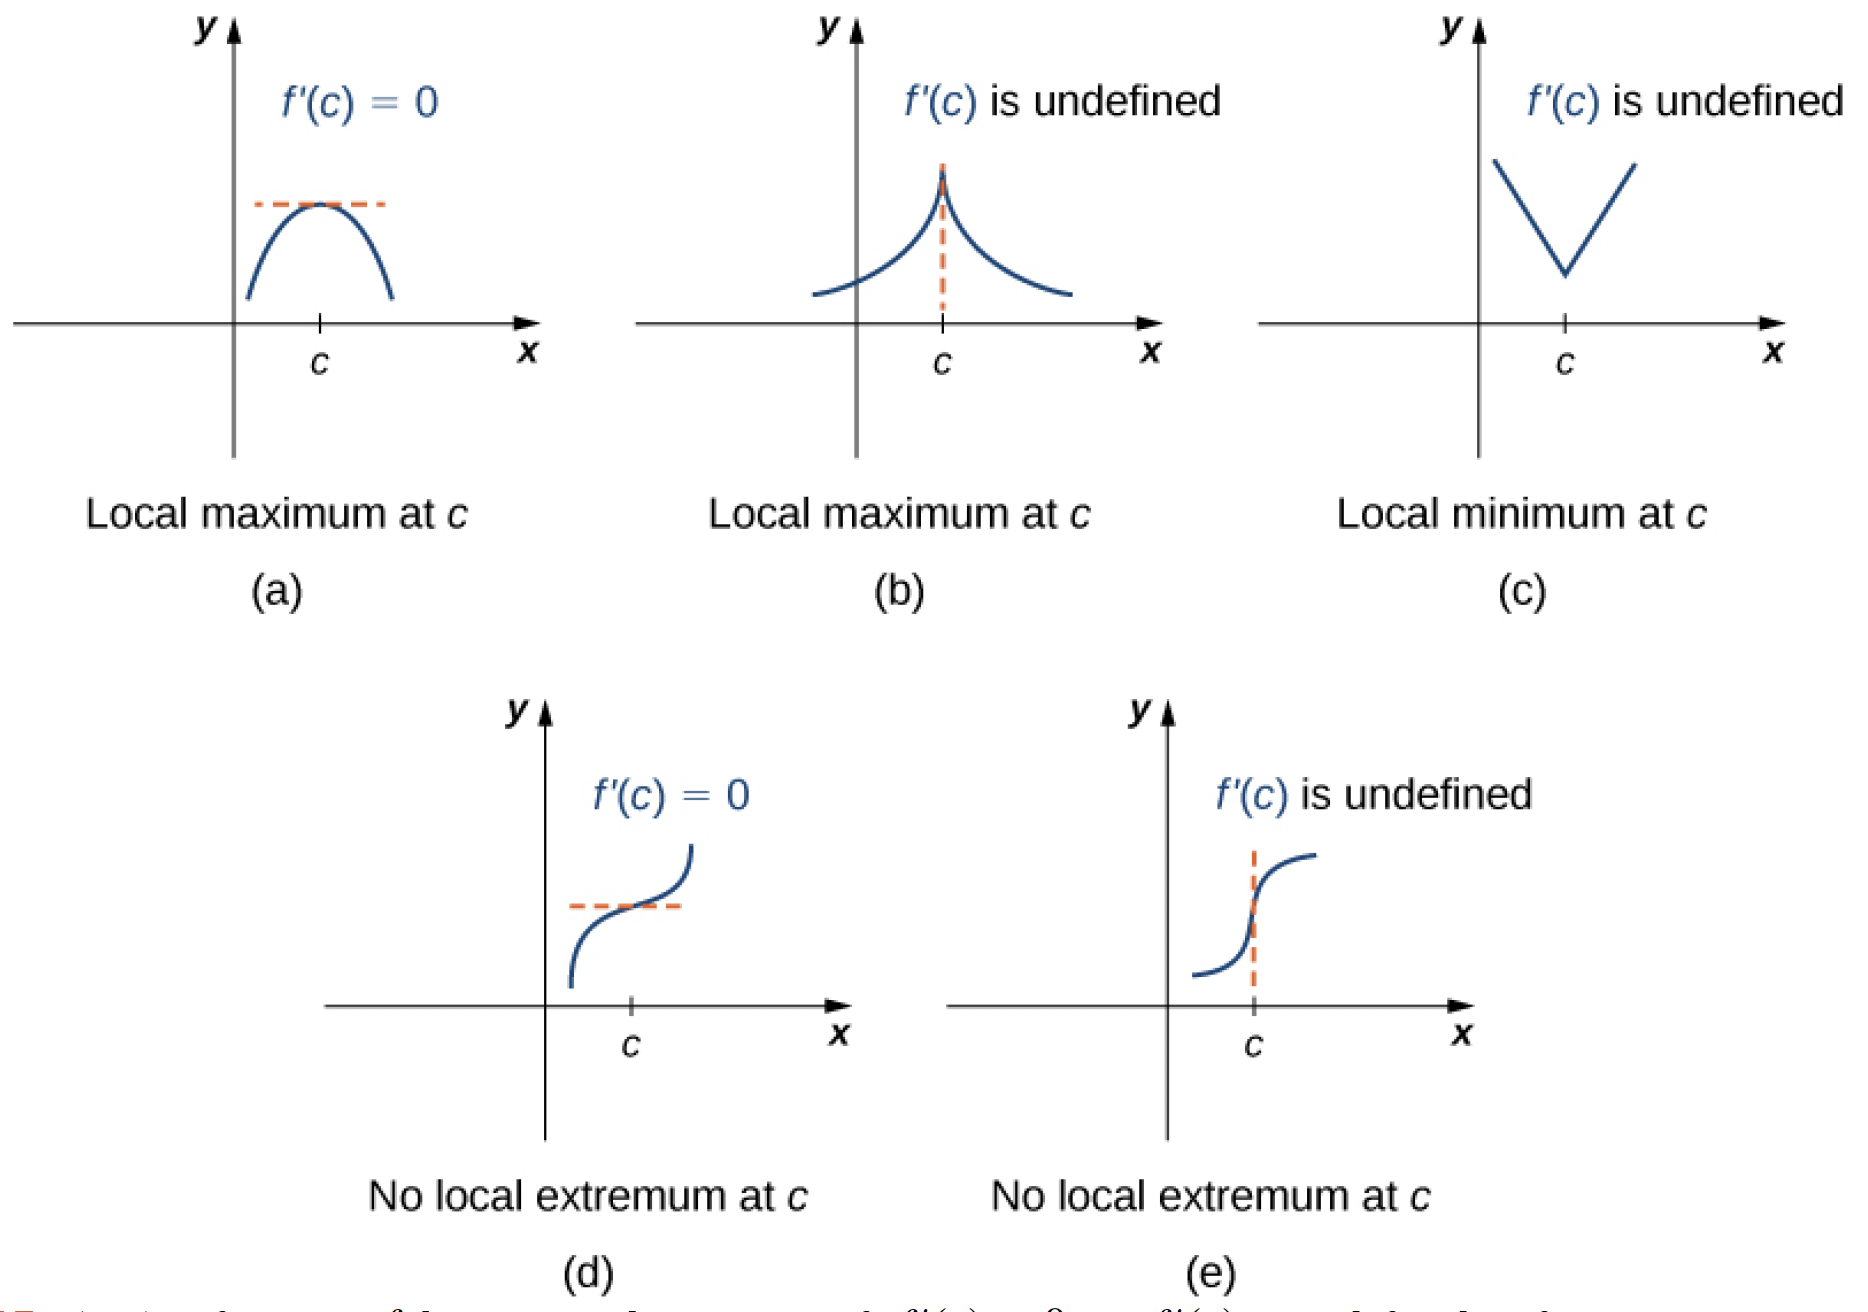
\includegraphics[width=0.75\textwidth]{images/optimization/critLocalExtreme.png}\footnotemark[1]
    \label{fig:critLocalExtreme}
\end{figure}
\footnotetext[1]{From \cite{openstax}; section 4.3 Maxima and Minima; Figure 4.15.}

%%%%%%%%%%%%%%%%%%%%%%%%%%%%%%%%%%%%%%
\begin{tcolorbox}[title = {The First Derivative Test for Extremes:}]

Suppose that $c$ is a \textbf{critical number} of a continuous function $f$. For each critical number $c$, examine the sign of $f'$ to the left and to the right of $c$. What happens to the sign as you move from left to right?
\renewcommand{\labelenumi}{(\alph{enumi})}
\begin{enumerate}[leftmargin=*]

    \item If $f'(x)$ changes from \textbf{positive to negative} at $c$, then $f$ has a \textbf{local max} at $(c,f(c))$.
    \item If $f'(x)$ changes from \textbf{negative to positive} at $c$, then $f$ has a \textbf{local min} at $(c,f(c))$.
    \item If $f'(x)$ \textbf{does not change sign} at $c$, then $(c,f(c))$ is \textbf{neither} a local max nor a local min.
\end{enumerate}
\end{tcolorbox}

\begin{tcolorbox}[title={Steps for finding where $f$ is Increasing/Decreasing or any Local Extrema}]
\begin{enumerate}[leftmargin=*]
    \item Find the \textbf{domain} of $f$.
    \item Find all \textbf{partition numbers} of $f'$.
    \item Find all \textbf{critical numbers} of $f$.
    \item Make a \textbf{sign chart} to track where $f'>0$ or $f'<0$ by following these steps:
    \renewcommand{\labelenumii}{(\roman{enumii})}
    \begin{enumerate}
        \item Plot all partition and critical numbers on a number line.
        \item Choose values to test regions on the number line around the critical/partition numbers.
        \item Plug test values into $f'$ and record the sign $(\pm)$
    \end{enumerate}
    \item Determine any \textbf{local extrema} using the \emph{First Derivative Test for Extremes}.
\end{enumerate}
\end{tcolorbox}

\begin{tcolorbox}[title={Locating Global Extrema Over An Open Interval}]
\noindent If you are trying to find a global max or min on an open interval (or the whole real line), and there is more than one critical point, then you need to look at the graph to decide whether there is a global max or min. \underline{Be sure that all your critical points show in your graph}, and that you go a little beyond – that will tell you what you want to know.
\end{tcolorbox}
%%% Question 11 from https://www.math.tamu.edu/~mayaj/m142_Chapter5_Sec5.1.pdf%%%
\begin{example}
Use the graph of the function $f(x)$ displayed below to answer the following questions.
\begin{figure}[h]
    \centering
    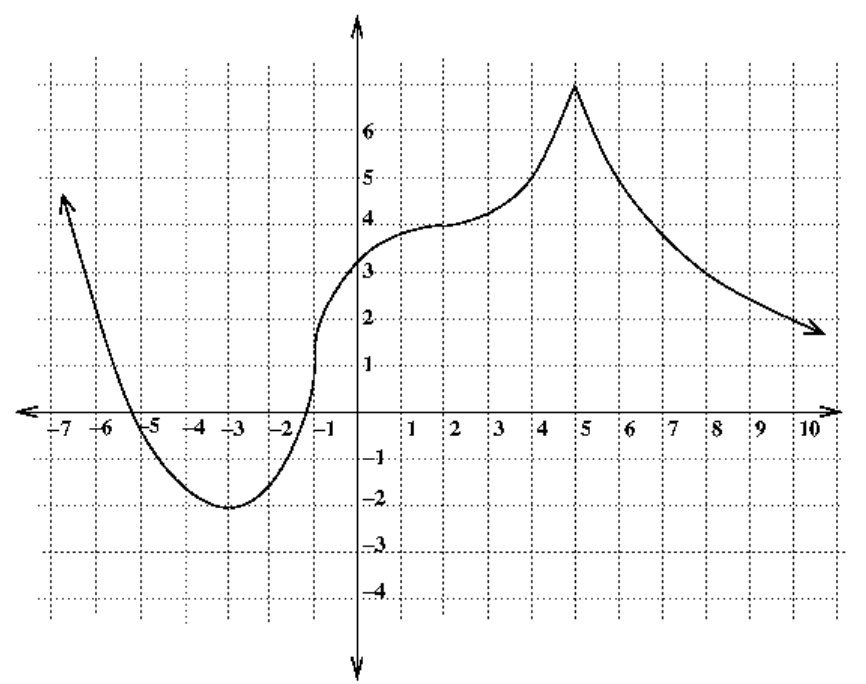
\includegraphics[width=0.6\textwidth]{images/optimization/exampleGraph1.png}
    \label{fig:my_label}
\end{figure}
\renewcommand{\labelenumi}{(\alph{enumi})}
\begin{enumerate}[leftmargin=*]
    \item Find the critical values where $f'(x)$ does not exist.\vspace{1cm}
    \item Find the critical values where $f'(x)=0$.\vspace{1cm}
    \item Find the $x-$coordinate(s) of the relative maxima for $f(x)$. \vspace{1cm}
    \item Find the $x-$coordinate(s) of the relative minima for $f(x)$. \vspace{1cm}
\end{enumerate}
    %%short answer
    \begin{sol}
    (a) $x=-1,5$ (b) $x=-3,2$ (c) $x=5$ (d) $x=-3$
    \end{sol}
    %%solution
    \begin{solL}
    Complete solution here.....
    
    \end{solL}
    
\end{example}

%% Question 9 from https://www.math.tamu.edu/~mayaj/m142_Chapter5_Sec5.1.pdf%%%
\begin{example}
Given the function $f(x)=\displaystyle\frac{x^2+3}{x-1}$ and its first derivative is shown below:
\begin{equation*}
    f'(x)=\frac{(x-3)(x+1)}{(x-1)^2}
\end{equation*}
Answer the following questions.
\renewcommand{\labelenumi}{(\alph{enumi})}
\begin{enumerate}[leftmargin=*]
    \item Find the domain of $f$. \vspace{1in}
    \item Find the partition number(s) of $f'$. \vspace{1in}
    \item Find the critical number(s) of $f$. \vspace{1cm}
    \item Make a sign chart for the function and use the chart to find the following:\vspace{0.75in}
    \renewcommand{\labelenumii}{(\roman{enumii})}
    \begin{enumerate}
        \item all intervals on which $f(x)$ is increasing.\vspace{1cm}
        \item all intervals on which $f(x)$ is decreasing.\vspace{1cm}
        \item the $x-$coordinate(s) of all relative extrema on the graph of $f(x)$. \vspace{1cm}
    \end{enumerate}
    
\end{enumerate}
    %%short answer
    \begin{sol}
    (a) $(-\infty,1)\cup (1,\infty)$ (b) $x=-1;x=1;x=3$ (c) $x=-1;x=3$ (d)(i) $(-\infty,-1)\cup (3,\infty)$ (d)(ii) $(-1,1)\cup (1,3)$ (d)(iii) local max at $x=-1$; local min at $x=3$
    \end{sol}
    %%solution
    \begin{solL}
    Complete solution here.....
    
    \end{solL}
    
\end{example}

%%%Example: Dave's handout 2.3 Derivatives: Behavior and graph of a function%%%
\begin{example}\label{1stDervTest}
For each of the following functions, determine all \textbf{local extrema} using the \emph{First Derivative Test}. Follow the \emph{Five Steps for finding where $f$ is increasing/decreasing or any local extrema}. Then, use the given graph of each function to help determine any \textbf{global extrema}.
\renewcommand{\labelenumi}{(\alph{enumi})}
\begin{enumerate}[leftmargin=*]
    \item $f(x)=\displaystyle\frac{1}{3}x^3-\frac{5}{2}x^2+4x$. %%OpenStax; 4.3 Maxima and Minima; ex.4.12a
    \begin{figure}[h!]
        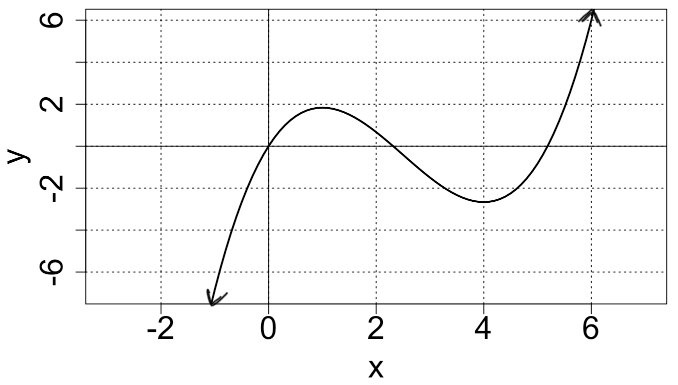
\includegraphics[width=0.45\textwidth,inner]{images/optimization/exampleGraph2.png}
        \label{fig:exampleGraph2}
    \end{figure}
    \newpage
    \item $f(x)=(x^2-1)^3$. %%OpenStax; 4.3 Maxima and Minima; ex.4.12b
    \begin{figure}[h!]
        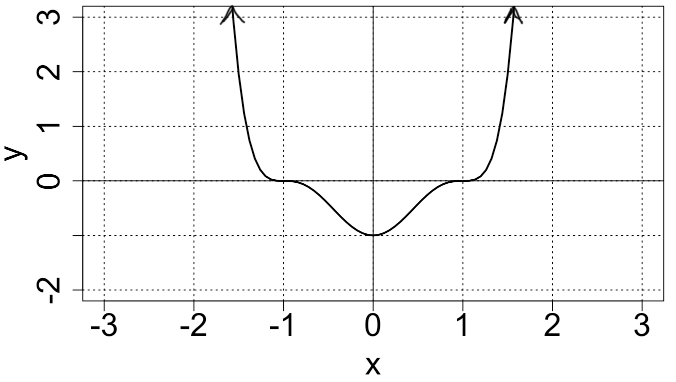
\includegraphics[width=0.45\textwidth,inner]{images/optimization/exampleGraph3.png}
        \label{fig:exampleGraph3}
    \end{figure}
     \vspace{1in}
    \item $f(x)=x+\displaystyle\frac{100}{x-1}$.  %%%Example: Dave's handout 2.3 Derivatives: Behavior and graph of a function%%%
    \begin{figure}[h!]
        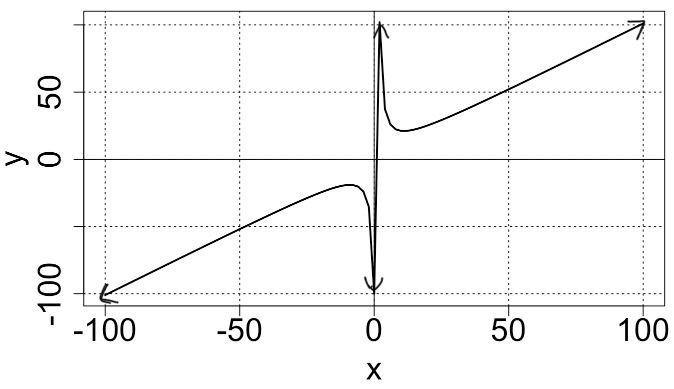
\includegraphics[width=0.45\textwidth,inner]{images/optimization/exampleGraph4.png}
        \label{fig:exampleGraph4}
    \end{figure}
     \vspace{1in}
    \item $f(x)=\displaystyle\frac{10}{x+2}$. %%%Example: Dave's handout 2.3 Derivatives:Behavior and graph of a function%%%
    \begin{figure}[h!]
        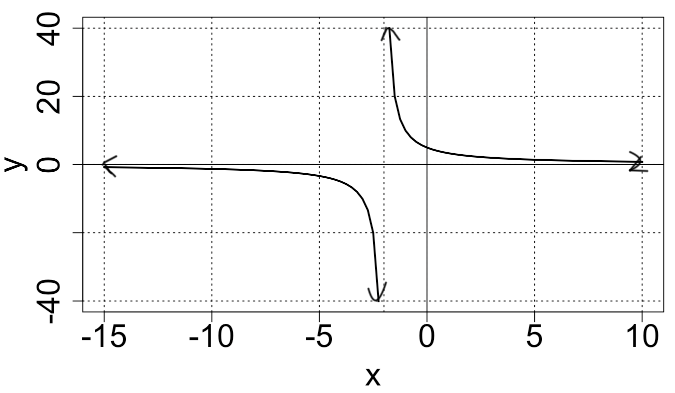
\includegraphics[width=0.45\textwidth,inner]{images/optimization/exampleGraph5.png}
        \label{fig:exampleGraph5}
    \end{figure}
     \vspace{1in}
\end{enumerate}
    %%short answer
    \begin{sol}
    (a) local max at $x=1$;local min at $x=4$;no global extrema. (b) only local (and global) minimum at $x=0$. (c) local max at $x=-9$; local min at $x=11$; no global extrema. (d) no extrema.
    \end{sol}
    %%solution
    \begin{solL}
    Complete solution here.....
    
    \end{solL}
    
\end{example}

\begin{tcolorbox}[title={Steps For Locating Global Extrema Over A Closed Interval}]
Consider a continuous function $f$ defined over the closed interval $[a, b]$.
\begin{enumerate}
    \item Evaluate $f$ at the endpoints $x=a$ and $x=b$.
    \item Find all critical points of $f$ that lie over the interval $(a,b)$ and evaluate $f$ at those critical points.
    \item Compare all values found in (1) and (2). Since \underline{the global extrema must occur at endpoints or critical points}, the largest of these values is the global maximum of $f$ . The smallest of these values is the global minimum of $f$ .
\end{enumerate}
\end{tcolorbox}

%%%Example: Calaway, Applied Calculus; section 2.7; Example 6%%%
\begin{example}
Given $f(x)=x^3-3x^2-9x+5$ for $-2\le x\le 6$, determine all \textbf{local extrema} using the \emph{First Derivative Test}. Follow the \emph{Five Steps for finding where $f$ is increasing/decreasing or any local extrema}. Then, use the steps described above to locate any \textbf{global extrema}.
    %%short answer
    \begin{sol}
    Local max of 10 at $x=-1$; local (and global) min of $-22$ at $x=3$; global max of $59$ when $x=6$.
    \end{sol}
    %%solution
    \begin{solL}
    Complete solution here.....
    
    \end{solL}
    
\end{example}
\vspace{0.6in}

%%%%%%%%%%%%End Examples%%%%%%%%%%%%%%%%%%
%%%%%%%%%%%%%%%End Topic%%%%%%%%%%%%%%%%%%
\newpage
\noindent The concavity of a function can also help us determine whether a critical point is a maximum or minimum or neither. For example, if a point is at the bottom of a concave up function, then the point is a minimum (see figure \ref{fig:oneLocalExtrema}). 
\begin{tcolorbox}[title={The Second Derivative Test for Extremes:}]
\begin{enumerate}[leftmargin=*]
    \item Find the \textbf{domain} of $f$.
    \item Find all \textbf{critical numbers} of $f$.
    \item For those critical points where $f'(c)=0$, find $f''(c)$.
    \item Locate any \textbf{local extrema} by determining the sign of $f''(c)$ as follows:
    \renewcommand{\labelenumi}{(\alph{enumi})}
    \begin{enumerate}[leftmargin=*]
        \item If $f''(c)<0$ then $f$ is \textbf{concave down} and has a \textbf{local maximum} at $x=c$.
        \item If $f''(c)>0$ then $f$ is \textbf{concave up} and has a \textbf{local minimum} at $x=c$.
        \item If $f''(c)=0$ then $f$ may have a local maximum, a minimum or neither at $x=c$.
    \end{enumerate}
\end{enumerate}
\end{tcolorbox}
\vspace{-0.25cm}
\begin{example}
\noindent Given $f(x)=x+\displaystyle\frac{100}{x-1}$, determine all \textbf{local extrema} by using the \emph{Second Derivative Test for Extremes} as described above. You may use the \emph{critical numbers} of $f$ that were already found in part c of Example \ref{1stDervTest}. Compare your results to the results from using \emph{First Derivative Test for Extremes} in the example. 
%%short answer
    \begin{sol}
    local max at $x=-9$; local min at $x=11$; same results.
    \end{sol}
    %%solution
    \begin{solL}
    Complete solution here.....
    
    \end{solL}
\end{example}
\vspace{2in}


%%%%%%%%%%%%%%%End Lesson%%%%%%%%%%%%%%%%%%
\Closesolutionfile{ans}
\Closesolutionfile{ansL}

%%%Short Answers to Examples%%%
\vspace*{\fill}
\subsection*{Short Answers to Examples}
%\vspace{-0.25cm}

\input{ans8}



